\documentclass[10pt]{article}

\usepackage{spheric}
%%%TITLE
\title{Developing an Extensible, Portable, Scalable Toolkit for massively parallel Incompressible Smoothed Particle Hydrodynamics (ISPH)}
\date{}

%%AFFILIATIONS
\author[1]{Xiaohu Guo$^\dagger$}
\author[2]{Benedict D. Rogers}
\author[2]{Steven Lind}
\author[2]{Peter K. Stansby}

\affil[1]{Hartree Centre, STFC, Daresbury Laboratory, WA4 4AD, UK}
\affil[2]{School of Mechanical, Aerospace and Civil Engineering, University of Manchester, M13 9PL, UK}

\affil[$\relax$]{\email{\dagger}{xiaohu.guo@stfc.ac.uk}}


%%DOCUMENT
\begin{document}

\maketitle

%\SelectedTopics{}

%%PLEASE PUT YOUR ABSTRACT HERE
\begin{abstract}
The stability, accuracy, energy conservation, boundary conditions of the projection based particle method such as ISPH \cite{lind2012incompressible} have been greatly improved \cite{gotoh2016current}. However, for applications requiring 100s of millions of particles from the perspective of computation and high performance software implementation \cite{dominguez2013optimization}, there are still many challenges compared with other particle based methods. These may potentially hinder the use and exploitation of these methods for the large-scale real engineering applications which generally involve highly complex, nonlinear and distorted flow. Solving such applications requires a large number of particles and this in turn demands distributed computing with accelerating paradigms. The domain decomposition and dynamic load balancing using the message passing interface (MPI) for irregular particles distribution and computational domains with complex geometries are extremely challenging to implement. An appropriate assignment of particles to processors and grouping physically-close particles within a single processor can greatly reduce communication overhead and improve the software scalability. The additional distinct challenge for projection-based particle methods is solving pressure Poisson equations (PPE). The added complexity for solving sparse linear equations for projection-based particle methods such as ISPH is that the sparsity of the matrix is changing every time step due to the particle movement and hence changing connectivity of the computation points.


In this work, we present our ISPH toolkit for massively parallel simulations which aims to resolve the above challenges and facilitate the projection-based particle-methods software development. We provide all the major performance critical `software kernels' such as the nearest neighbour list searching kernel using cell linked list approach, the domain decomposition, dynamic load balancing and particles ordering kernels using Hilbert Space Filling Curve and the PPE solver using the open-source high-performance computing (HPC) library PETSc. The innovations of the new ISPH toolkit are summarised in the following:
\begin{itemize}
\item Data structures designed to organise multiple kinds of fluid particles together with different boundary particles to maximise data locality and cache reuse. This enables software extensibility and communication between highly irregular subdomains.
\item Domain decomposition and dynamic load balancing particularly for irregular particle distributions and computational domains with complex geometries. Figure \ref{fig:11-1} gives example of initial domain decomposition for the SPHERIC test case 2 Kleefsman's dambreaking test-case.
\item Flexible parallel communication algorithms to manage efficiently specific tasks for user software development including updating halos, boundaries in the form of a single velocity vector, or new variables defined by users.
\item Particle ordering in order to group physically-close particles which improves performance on cache-based computing architectures.
\item Improved ISPH boundary conditions with general applicability and attractive accuracy versus performance which facilitates
application development.
\item Flexibility using different sparse linear solvers for different applications (PETSc) by improving the structure of the PPE matrix by preconditioning with particle reordering.
\end{itemize}
Detailed performance analysis using ISPH for each performance software kernels demonstrate our toolkit scalability (see Figure \ref{fig:11-2}) of using tens of thousands cores to solve complex, nonlinear and distorted flow with ISPH. The analysis has revealed the parts of the code that are highly efficient and those that become a potential bottle neck as the number of processes increases beyond 10,000. The implementation details are intended to form future guidance for the new projection-based particle application development.

\begin{figure}[!htb]
\begin{minipage}[b]{0.46\linewidth}
\centering
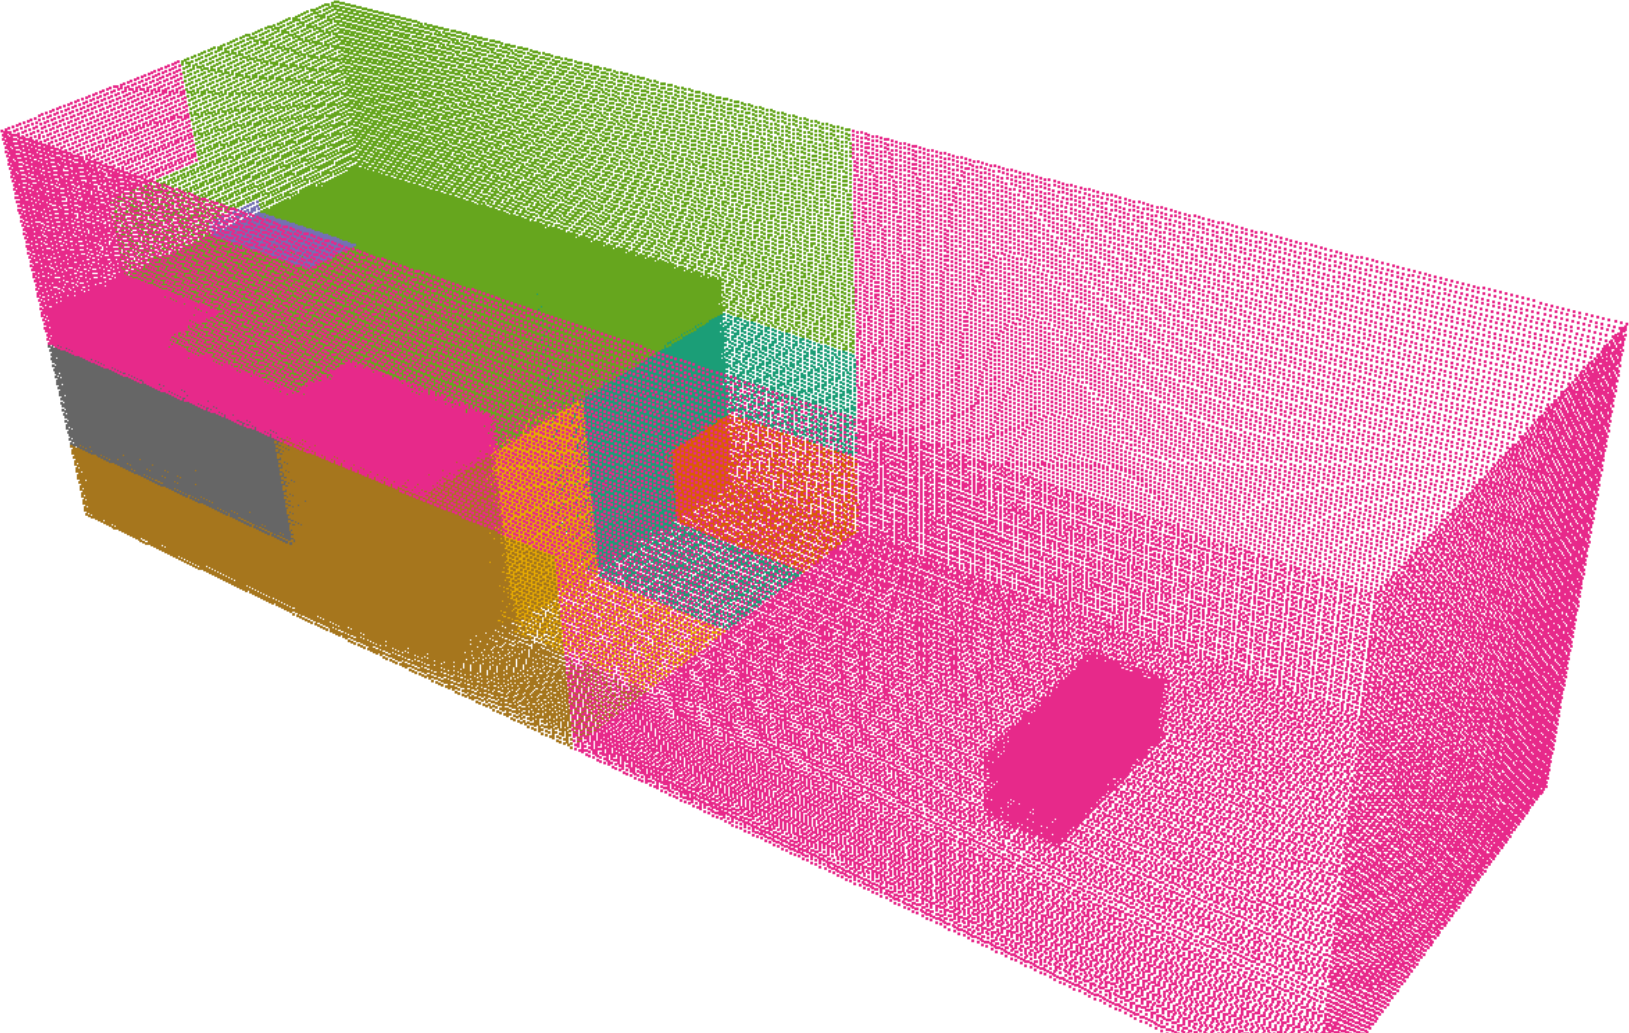
\includegraphics[width=0.85\textwidth]{11-11.png}
\caption{3D domain decomposition with HSFC with 8 MPI Tasks, different colours represent different partitions}\label{fig:11-1}
\end{minipage}
\begin{minipage}[b]{0.05\linewidth}
~
\end{minipage}
\begin{minipage}[b]{0.46\linewidth}
\centering
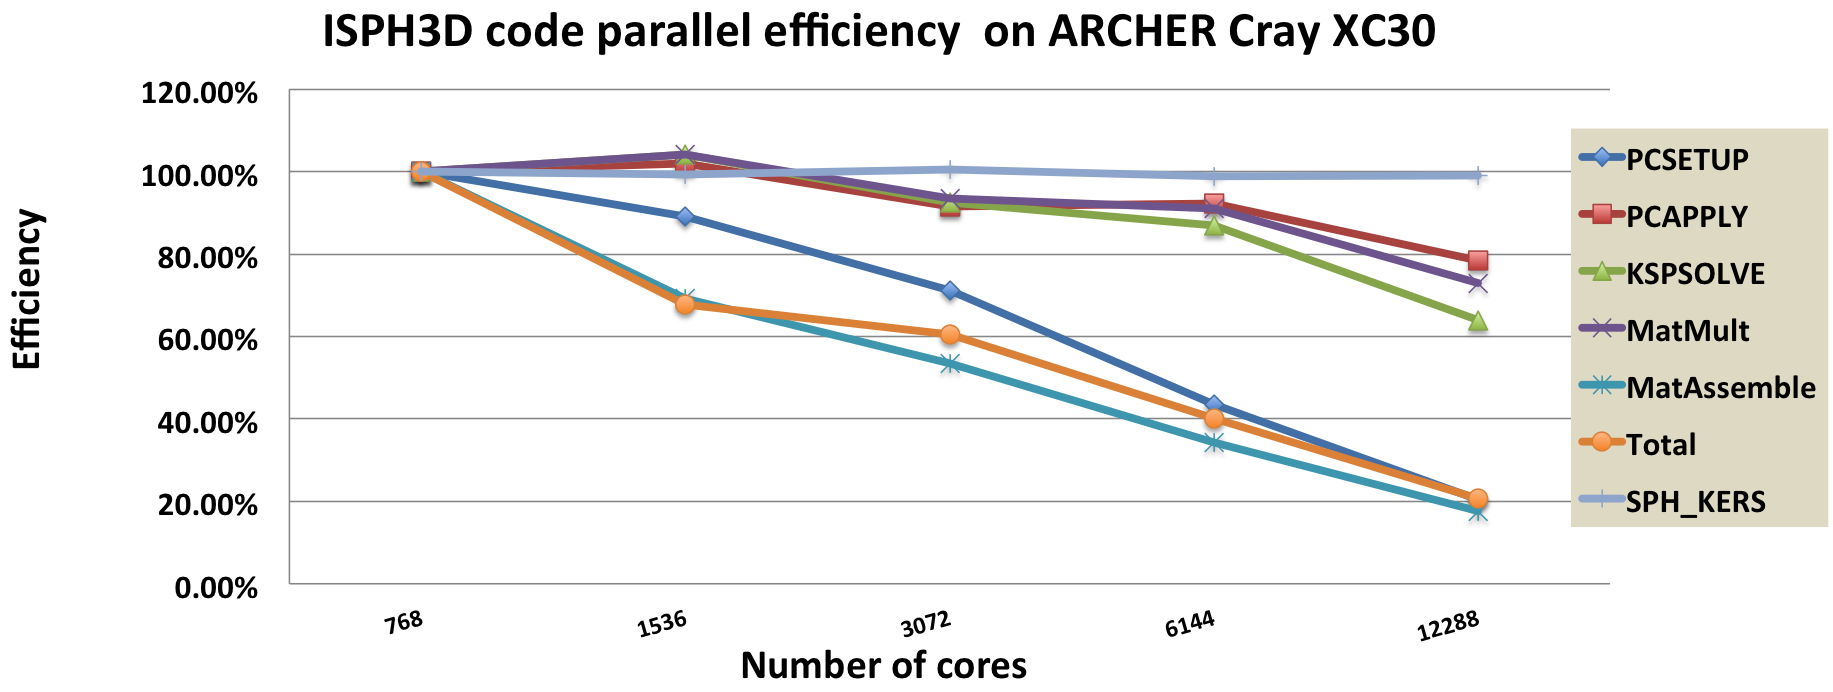
\includegraphics[width=\textwidth]{11-21.png}
\caption{Efficiency Performance Analysis for ISPH3D}\label{fig:11-2}
\end{minipage}
\end{figure}


\end{abstract}


%%THE END OF ABSTRACT

\addbib

\end{document}
